\documentclass[11pt]{article}
\usepackage[margin=1in]{geometry}
\usepackage{amsmath,amssymb,bm}
\usepackage{booktabs,tabularx,array}
\usepackage{graphicx,float}
\usepackage{longtable}
\usepackage{listings}
\usepackage{algorithm,algpseudocode}
\usepackage{tikz}
\usetikzlibrary{arrows.meta,positioning}
\usepackage[hidelinks]{hyperref}
\newcommand{\vb}[1]{\bm{#1}}
\newcommand{\sk}{\operatorname{sk}}
\newcommand{\Frame}{\operatorname{Frame}}
\newcommand{\Exp}{\operatorname{Exp}}
\newcommand{\Log}{\operatorname{Log}}
\newcommand{\R}{\mathbb R}
\newcolumntype{Y}{>{\raggedright\arraybackslash}X}
\renewcommand{\algorithmicrequire}{\textbf{Input:}}
\renewcommand{\algorithmicensure}{\textbf{Output:}}
\lstset{basicstyle=\ttfamily\footnotesize,breaklines=true,columns=fullflexible}
\title{CIS 1 Assignment 2 Report}
\author{Bader Al-Salhabi \\ JHED ID: 49CD6F
\and Yinxiang Luo \\ JHED ID: yluo87}
\date{October 2026}
\begin{document}
\maketitle
\begin{center}
We have followed the rules in completing this assignment.\\[6pt]
Signatures:\\
\IfFileExists{Bader's Signature.jpeg}{
\includegraphics[width=.3\linewidth]{Bader's Signature.jpeg}}{\rule{5cm}{.4pt}}\\
Bader Al-Salhabi\\[12pt]
\IfFileExists{Will's Signature.jpeg}{
\includegraphics[width=.3\linewidth]{Will's Signature.jpeg}}{\rule{5cm}{.4pt}}\\
Yinxiang Luo
\end{center}
\setcounter{tocdepth}{1}

\newpage
\tableofcontents
\clearpage
\section{Summary}
We calibrate a Cartesian robot with a spherical wrist using an optical tracker and an exactly manufactured end-effector calibration body. Encoder values alone do not describe the actual motion accurately because the joint axes, joint displacement maps, tool mounting, and base placement differ from their nominal values. We use the handout's parameter-estimation route rather than a dense six-dimensional workspace map \cite{handout}. The derivation follows the authors' handwritten frame, residual, and Jacobian analysis \cite{notes}. Individual-axis sweeps supply observations for a joint fit of the base, axes, tool, and smooth joint distortion. The resulting forward model also supports numerical inverse kinematics.

The acceptance targets are a position error of at most $0.2$~mm and an orientation error of at most $10^{-3}$~rad. These are checked using maximum errors, in addition to RMS statistics. In controlled report-validation runs, robot seeds 1 and 2 both meet the targets on the 729-pose forward grid and 40 inverse targets per seed. This is empirical validation on the stated test set, not a proof over the continuous workspace. The fitted Jacobian has effective rank $33/34$, so accurate predictions do not imply unique recovery of all physical parameters. The current test suite passes all 37 tests, including ordinary-marker refinement; Section~\ref{sec:tests} describes the checks.

\section{Design}
\subsection{Frames, scene, and calibration body}
We write ${}^{A}F_B=[R,p]$ for a transform mapping point coordinates from frame $B$ to frame $A$: $p^A=Rp^B+p$. Let $W,T,B,E$ denote workspace, tracker, robot base, and end effector. The tracker returns $Y_j={}^{T}F_{E,j}$ because the special calibration body's coordinate system exactly coincides with $E$ \cite{handout,frames}. Define
\begin{equation}
 F_X={}^{T}F_B=({}^{W}F_T)^{-1}{}^{W}F_B,
 \qquad Y_j\approx F_X F_{ee}(\theta_j).
 \label{eq:closure}
\end{equation}
This closes two paths to the same end effector; the robot itself is a serial kinematic chain.

\begin{table}[H]\centering\small
\caption{Scene and design choices. All lengths are in mm.}
\begin{tabularx}{\linewidth}{@{}lY@{}}\toprule
Quantity & Selected value and reason\\\midrule
Tracker pose & ${}^{W}F_T=[I,(0,0,0)^T]$; viewing direction is local $+z$.\\
Approximate robot base & ${}^{W}F_{B,\mathrm{approx}}=[I,(-800,0,1400)^T]$; actual placement is perturbed by the simulator.\\
Calibration markers & $(75,0,0),(-75,0,0),(0,0,75),(0,0,-75)$ in $E$. Each has radius 75 and the layout is non-collinear.\\
Visibility check & 81 selected joint configurations before collection; all 81 are nominally visible for the selected scene.\\
Baseline & 10 configurations: a central pose, translations about it, and three wrist excitations.\\
Main plan & 53 distinct configurations, 186 move/sample entries including repeated readings and returns.\\
Default spacing & At most 100~mm for translation and 0.5~rad for wrist sweeps; three consecutive entries per accepted configuration.\\\bottomrule
\end{tabularx}\end{table}

The four markers are coplanar, but not collinear; known point correspondences determine a proper rigid rotation. A non-coplanar body is not required for this registration problem. The spread at the allowed radius improves rotational sensitivity. The tracker model does not include a separate marker-occlusion model. Visibility checks use nominal geometry and do not establish a worst-case clearance guarantee under installation errors.

\subsection{Error budget and sampling trade-off}
The tracker has 0.1~mm per-coordinate marker noise, bounded systematic error, and no pose jiggle for this assignment. Random error can be reduced by repeated independent observations; a systematic field cannot be removed by averaging at one pose. Robot motion also has repeatability noise: $0.005$~mm on the linear joints and $10^{-4}$~rad on the wrist joints \cite{handout}. The calibration is deterministic in its mean predictions and does not predict each noise realization.

For centered marker positions $a_k$, small rotational measurement uncertainty is related to
\begin{equation}
 C_\alpha\approx\sigma_b^2\left[\sum_k\bigl(\|a_k\|^2I-a_ka_k^T\bigr)\right]^{-1}.
 \label{eq:markerinfo}
\end{equation}
This follows from linearizing each point's rotation sensitivity as $-[a_k]_\times$ and forming the least-squares normal matrix \cite{calibration}. For our layout the information matrix inside brackets is
\[\operatorname{diag}(11250,22500,11250)\;\mathrm{mm}^2.\] The largest coordinate standard deviation is approximately $9.43\times10^{-4}$~rad for one reading and $5.44\times10^{-4}$~rad for three independent readings. These are local random-noise estimates, not bounds on the final model's orientation norm.

If a scalar distortion $g$ is Lipschitz with slope bound $L$, linear interpolation across an interval of length $h$ has error at most $Lh/2$: at $x=\lambda h$, the bound is $2Lh\lambda(1-\lambda)\le Lh/2$. A robot linear-joint bound $L=5\times10^{-4}$ and $h=100$~mm gives 0.025~mm per joint. A wrist bound $L=5\times10^{-5}$ and $h=0.5$~rad gives $1.25\times10^{-5}$~rad. However, our fitted model is a global quadratic, not piecewise linear interpolation, and tracker distortion also contributes. Therefore these estimates motivate spacing but do not prove our fit meets the target. The planner scales its default spacing by $\min(1,\texttt{desired\_accuracy}/10^{-3})$; the repeat count remains separately configurable. These are initial design rules validated empirically, not an optimal sampling theorem.

\section{Mathematical Approach}
\subsection{Nominal and corrected forward kinematics}
The nominal model from the handout is \cite{handout}
\begin{align}
 F_{ee}(\theta)&=F_c(\theta)F_{cw}F_w(\theta)F_{we},\\
 F_c&=\Frame\left(I,\sum_{k=1}^3\theta_kd_k\right),\\
 F_w&=\Frame\left(R(n_4,\theta_4)R(n_5,\theta_5)R(n_6,\theta_6),0\right),\\
 F_{cw}&=\Frame(I,[500,0,0]^T),\qquad
 F_{we}=\Frame(I,[100,0,0]^T).
\end{align}
The nominal axes are $d_1,d_2,d_3=x,y,z$ and $n_4,n_5,n_6=x,y,z$. We use $d_4,d_5,d_6$ as shorthand for the wrist axes. At zero nominal joints, $F_{ee}(0)=[I,(600,0,0)^T]$. The apparent $\theta_s$ in the printed handout is interpreted as $\theta_2$. No separate $F_{cw}$ error is included in the supplied model.

The physical joint model is $\theta_k^*=\theta_k+\delta_{k,\mathrm{sys}}(\theta_k)+\delta_{k,\mathrm{rnd}}$. At physical home, $\theta_k^*=0$, giving the estimate
\begin{equation}
 \widehat\delta_{k,\mathrm{home}}=-\frac1H\sum_{h=1}^H\theta_{k,\mathrm{home}}^{(h)},\qquad H=5.
 \label{eq:home}
\end{equation}
We approximate the remaining smooth distortion with
\begin{equation}
 q_k=\theta_k+\widehat\delta_{k,\mathrm{home}}+
 \sum_{\ell=1}^{2}c_{k\ell}(\theta_k/s_k)^\ell,
 \quad s_k=\max(|\theta_{k,\min}|,|\theta_{k,\max}|).
 \label{eq:q}
\end{equation}
The constant term is fixed by homing, not freely fitted again. The quadratic is an approximation, not an assertion that the unknown distortion is exactly polynomial.

For $k=2,\ldots,6$, choose the two components of $\phi_k$ perpendicular to the nominal axis and define
\begin{equation}
 \widehat d_k=\exp([\phi_k]_\times)d_k,\qquad \widehat d_1=d_1.
\end{equation}
For an $x$ axis, for example, $\phi_k=(0,\phi_{ky},\phi_{kz})^T$. This avoids introducing the unobservable rotation about an axis that would leave that axis unchanged. Our corrected kinematics are
\begin{align}
 \widehat F_c&=\Frame(I,q_1d_1+q_2\widehat d_2+q_3\widehat d_3),\\
 \widehat F_w&=\Frame(R(\widehat d_4,q_4)R(\widehat d_5,q_5)R(\widehat d_6,q_6),0),\\
 \widehat F_{we}&=F_{we}\Exp(\xi_{we}^{\wedge}),\qquad
 \widehat F_X=F_{X,\mathrm{init}}\Exp(\xi_X^{\wedge}),\\
 \widehat F_{ee}&=\widehat F_c F_{cw}\widehat F_w\widehat F_{we}.
 \label{eq:corrected}
\end{align}
For $\xi=[\alpha^T,\rho^T]^T$, $\xi^\wedge=\left[\begin{smallmatrix}[\alpha]_\times&\rho\\0&0\end{smallmatrix}\right]$ and $\Exp(\xi^\wedge)=[\exp([\alpha]_\times),J_l(\alpha)\rho]$. Thus $\rho$ is not exactly the resulting translation except in the zero-rotation limit. These frame and small-perturbation constructions follow the course's calibration treatment \cite{frames,calibration}.

\begin{table}[H]\centering\small
\caption{The 34 fitted parameters; Python slices are half-open.}
\begin{tabular}{@{}llll@{}}\toprule
Block & Slice & Count & Meaning\\\midrule
$\xi_X$ & \texttt{0:6} & 6 & Base correction\\
$\tau=(\phi_2,\ldots,\phi_6)$ & \texttt{6:16} & 10 & Two tilt components per axis\\
$\xi_{we}$ & \texttt{16:22} & 6 & Tool correction\\
$c$ & \texttt{22:34} & 12 & Two distortion coefficients per joint\\\bottomrule
\end{tabular}\end{table}

\subsection{Point registration, frame averaging, and refinement}
Our registration implementation also draws on Jingnan Shi's explanation and Python implementation of Arun's method \cite{shi_arun}.
For corresponding points, solve $\min_{R\in SO(3),p}\sum_i\|Ra_i+p-b_i\|^2$. Center the points, form $H=\sum_i(a_i-\bar a)(b_i-\bar b)^T=U\Sigma V^T$, and obtain \cite{rigid,shi_arun}
\begin{equation}
 R=V\operatorname{diag}(1,1,\det(VU^T))U^T,\qquad p=\bar b-R\bar a.
\end{equation}
At least three non-collinear corresponding points are required. Centered rank below two is rejected. Coplanar rank-two data are valid; one zero singular value alone does not make this configuration invalid. The determinant correction excludes reflections. An orthogonal SVD result has determinant $+1$ or $-1$, not zero; degeneracy is diagnosed through input rank, rather than treating $\det(R)=0$ as a valid rotation case.

To average estimates $F_j=[R_j,p_j]$, set $\bar p=N^{-1}\sum_jp_j$, $M=N^{-1}\sum_jR_j=U\Sigma V^T$ and
\begin{equation}
 \bar R=U\operatorname{diag}(1,1,\det(UV^T))V^T.
 \label{eq:avg}
\end{equation}
This minimizes the chordal rotation objective $\sum_j\|R-R_j\|_F^2$; it is not claimed to be a geodesic rotation mean. It suits repeated estimates of one pose.

For an ordinary marker body, estimate its pose $G_j$ from each observation and average local points $\bar a_k=N^{-1}\sum_jG_j^{-1}b_{jk}$. The layout is determined only up to a rigid transform, so validation first aligns the estimated and actual layouts. This optional refinement is not used for our exact end-effector body. Its corrected implementation uses the returned point objects directly and passes the layout-improvement and sampling-time test.

\subsection{Initial base registration and nonlinear fitting}
A sample gives $F_{X,j}=Y_jF_{ee,\mathrm{nom}}(\theta_j)^{-1}$. We average these transforms using Eq.~\eqref{eq:avg}. The 10-sample estimate $F_{X,\mathrm{baseline}}$ diagnoses the initial model; the main-data estimate $F_{X,\mathrm{nom}}$ is passed to the model as $F_{X,\mathrm{init}}$. They describe the same frame relationship but use different data.

For fixed data $(\theta_j,Y_j)$ and candidate $\beta\in\R^{34}$, define
\begin{align}
 h(\theta_j;\beta)&=\widehat F_X(\beta)\widehat F_{ee}(\theta_j;\beta),\\
 E_j(\beta)&=Y_j^{-1}h(\theta_j;\beta)=[R_{e,j},p_{e,j}],\\
 r_j(\beta)&=\begin{bmatrix}\Log_{SO(3)}(R_{e,j})/10^{-3}\\p_{e,j}/0.2\end{bmatrix},\quad
 r(\beta)=\begin{bmatrix}r_1(\beta)\\\vdots\\r_N(\beta)\end{bmatrix},\\
 \widehat\beta&=\arg\min_\beta\frac12\|r(\beta)\|^2.
 \label{eq:objective}
\end{align}
Here $\Log_{SO(3)}$ returns a three-vector. Scaling uses acceptance tolerances rather than a measured noise covariance, so this is not claimed to be statistically optimal whitening. Rotations and coupled transforms make the fit nonlinear. Locally,
\begin{equation}
 r(\beta^{(t)}+\Delta\beta)\approx r(\beta^{(t)})+J_t\Delta\beta,
 \quad J_t=\left.\frac{\partial r}{\partial\beta}\right|_{\beta^{(t)}}.
\end{equation}
The Gauss--Newton interpretation is a local least-squares problem in $\Delta\beta$. The actual implementation calls SciPy's default trust-region reflective solver with no explicit bounds. It controls the step and stops when its convergence criteria are met. This is analogous to nonlinear reprojection refinement in camera calibration \cite{cv}; neither convergence nor a small total cost proves global optimality or pointwise acceptance.

\subsection{Jacobian rank and gauge freedom}
After fitting, we independently approximate the Jacobian by central differences:
\begin{equation}
 J_{:,k}\approx\frac{r(\widehat\beta+h_ke_k)-r(\widehat\beta-h_ke_k)}{2h_k},\qquad
 h_k=10^{-6}\max(1,|\widehat\beta_k|).
\end{equation}
With 186 samples, $J\in\R^{1116\times34}$. For $J=U\Sigma V^T$, the code reports
\begin{equation}
 \operatorname{rank}_{\mathrm{eff}}J=\#\{i:\sigma_i>10^{-6}\sigma_1\}.
\end{equation}
Both tested seeds give rank 33. A weak right singular vector $v$ satisfies $Jv\approx0$, so $r(\beta+\delta v)\approx r(\beta)$. This concerns a combination of parameters, not specifically parameter 34.

The model admits a base-coordinate gauge: for a rotation $G$ about the fixed first axis, a common rotation of the remaining axes and tool can be offset by $F_X'=F_XG^{-1}$, producing $F_{ee}'=GF_{ee}$ and therefore $F_X'F_{ee}'=F_XF_{ee}$. The fixed offsets along $x$ commute with this rotation. Locally this explains a redundant direction. Consequently raw fitted tilts and tool twists can differ substantially from truth despite accurate pose prediction. Axis-to-axis angles are invariant under a common base rotation and are more meaningful debug comparisons. The current code reports, but does not remove, this gauge. A future constrained fit should fix a suitable reference degree of freedom. Effective rank also depends on scaling and the numerical threshold.

As an optional investigation, we tested all 34 choices of a single fixed parameter in a separate source-code copy, without changing the submitted calibration model. Appendix~\ref{app:fixed-parameters} compares reduced-Jacobian ranks at the same fitted point and independent fits with each parameter fixed to zero. Multiple different constraints restore effective full column rank, so this exploration identifies candidate gauge constraints rather than a unique redundant parameter. The main model and all main performance results retain the original 34-parameter fit and its rank $33/34$.

\subsection{Inverse kinematics and error metrics}
The provided inverse solver numerically refines nominal wrist-branch solutions using $\widehat F_{ee}$. For a base-frame target $F$, it reduces
\begin{equation}
 \Delta F(\theta)=\widehat F_{ee}(\theta)^{-1}F
 =[\Delta R(\theta),\Delta p(\theta)],\qquad
 e(\theta)=\begin{bmatrix}\Log_{SO(3)}(\Delta R(\theta))\\\Delta p(\theta)\end{bmatrix}.
\end{equation}
using finite-difference derivatives and damped steps; it selects an in-limit branch near the supplied seed. Tests compare resulting poses, since joint solutions need not be unique. The inherited solver's limit check alone is not a general convergence certificate, so actual arrival error is measured independently.

For any reference $A$ and prediction $B$, let $D=A^{-1}B$. We report
\begin{equation}
 e_R=\|\Log_{SO(3)}(D_R)\|_2,\quad e_p=\|D_p\|_2,\quad
 \mathrm{RMS}(e)=\sqrt{N^{-1}\sum_je_j^2},\quad e_{\max}=\max_je_j.
 \label{eq:metrics}
\end{equation}
These errors are invariant under a common left coordinate transform because $(GA)^{-1}(GB)=A^{-1}B$ \cite{frames}.

\section{Algorithmic Approach}
The implementation uses Python, NumPy for arrays/SVD, SciPy for nonlinear least squares, and the supplied frame and simulation classes. Calibration uses public encoder, motion, and tracker interfaces. Ground truth is read only for debugging and evaluation, never for fitting or pose-plan selection.

\subsection{Module-level algorithms}
The following summaries describe the student implementation in execution terms. The mathematical equations above define the objectives; these steps explain how each module computes its outputs. Function interfaces and file dependencies are listed separately in Section~\ref{sec:program-structure}.

\subsubsection{Error measurement: \texttt{metrics.py}}
\begin{enumerate}
\setlength{\itemsep}{0pt}
\item \texttt{frame\_error(A,B)} computes $D=A^{-1}B$, extracts the rotation vector from $D_R$ using \texttt{log\_so3}, and returns its Euclidean norm and the norm of $D_p$. The result is an angle in rad and a distance in mm.
\item \texttt{summarize\_errors(errors)} rejects an empty sequence, converts the pairs to a two-column array, and computes the count, RMS, and maximum independently for each column. It returns a statistics dictionary without changing the input observations.
\end{enumerate}

\subsubsection{Registration and averaging: \texttt{registration.py}}
\begin{enumerate}
\setlength{\itemsep}{0pt}
\item \texttt{register\_points(a,b)} checks matching counts and at least three pairs, converts the point lists to $3\times N$ arrays, and subtracts their centroids. It rejects centered point sets of rank below two, forms $H=A'B'^T$, and computes its SVD. Apply the determinant correction to obtain $R\in SO(3)$, recover $p=\bar b-R\bar a$, and return the source-to-target frame. This is our implementation, not a call to the simulator's registration solver.
\item \texttt{average\_frames(frames)} rejects an empty list, averages the translation vectors, and averages the rotation matrices elementwise into $M$. Project $M$ onto $SO(3)$ using SVD with the determinant correction, then combine the projected rotation and mean translation into a frame.
\item \texttt{refine\_marker\_body(trk,placed,n)} keeps the nominal layout fixed during collection. For each of $n$ snapshots, obtain the observed points and raise an error if the body is invisible. Register nominal points to observed points, transform the observations back with the inverse fitted frame, and store the resulting local coordinates. Average each marker across snapshots, update the body's nominal layout once, and return the new point list. Hidden manufactured geometry is never used by this algorithm; it is used only by its test.
\end{enumerate}

\subsubsection{Collection and initial registration: \texttt{workflow.py}}
\begin{enumerate}
\setlength{\itemsep}{0pt}
\item \texttt{measure\_home\_offsets(rob,H)} performs $H$ physical homings, copies each six-component encoder reading, averages by joint, and negates the result. This supplies fixed home corrections for the later model.
\item \texttt{plan\_calibration\_poses(...)} selects default or user-specified spacing, repetition count, and reference joint vector. For each joint, generate an endpoint-inclusive grid using \texttt{linspace}, with the number of intervals chosen by the ceiling of range/spacing. Start at the endpoint nearer the reference, vary only this joint, and return to reference before the next sweep. The local \texttt{append\_pose} helper checks finite values, joint limits, and nominal marker visibility before copying repeated entries into the plan; it avoids duplicate adjacent blocks. Planning does not move the robot or advance simulated time.
\item \texttt{collect\_calibration\_data(...)} records the initial simulated clock and visits each absolute joint vector. Move once, then perform the requested number of snapshots, retrieving the calibration body's tracker-frame pose after each. An invisible observation raises an error rather than silently entering invalid data. Store paired joint copies and frames in \texttt{CalibrationData}, then record elapsed simulated time. The data container also provides its observation count through \texttt{\_\_len\_\_}.
\item \texttt{estimate\_base\_frame(data,kins)} checks nonempty, equally sized joint/frame lists. For each pair compute $Y_j\,\texttt{kins.fwd\_kins}(\theta_j)^{-1}$, then call \texttt{average\_frames} on those base estimates. The same routine serves the baseline and main collections.
\end{enumerate}

\subsubsection{Model, fitting, and diagnostics: \texttt{kinematics.py}}
\begin{enumerate}
\setlength{\itemsep}{0pt}
\item The \texttt{ImprovedKinematics} constructor copies nominal limits and timing settings, stores the initial base frame and measured home offsets, and calls \texttt{initial\_params()} to create $22+6n_{\mathrm{poly}}$ zero corrections (34 for degree two). Nonzero measured home offsets remain active even when these corrections are zero.
\item \texttt{base\_frame(params)} maps the first six parameters through \texttt{exp\_se3} and right-multiplies this correction onto the initial base estimate.
\item \texttt{fwd\_kins(theta,params)} applies the measured home offsets and normalized polynomial corrections to all six joints. Construct the five tilted unit axes from their two-component rotation vectors, leaving the first axis fixed. Sum the three corrected translations, multiply the three wrist rotations in order, apply the tool correction, and compose the corrected chain. Its output remains in robot-base coordinates. \texttt{predict\_in\_tracker} left-multiplies it by \texttt{base\_frame}.
\item \texttt{residuals(params,data)} predicts each recorded pose, forms observed-inverse times prediction, and concatenates its rotation-vector and translation components after scaling by the two target tolerances. \texttt{fit(data)} passes this vector function to \texttt{least\_squares}, stores the returned parameters, and reports solver status, cost, evaluation count, and termination message. It does not acquire new data during optimization.
\item The provided \texttt{inv\_kins(F,seed)} generates nominal wrist-branch initial guesses and refines each using finite-difference pose derivatives and damped, step-limited updates. Its local \texttt{pose\_delta} helper computes the six-component target-relative pose residual used by these updates. It wraps the appropriate wrist angles, retains in-limit candidates, and selects the one nearest \texttt{seed}. The current code does not perform a final residual acceptance check before retaining a candidate; our arrival trials therefore measure actual error separately rather than treating a returned joint vector as a convergence guarantee.
\item \texttt{jacobian\_rank\_report(data)} perturbs each parameter positively and negatively, builds the central-difference Jacobian, applies SVD, and returns the effective rank, singular values, threshold, and weak right-singular directions. This is a post-fit diagnostic, separate from the optimizer's internal Jacobian estimation.
\item \texttt{parameters\_report()} reconstructs axes and tilts, computes all pairwise axis angles, and reports the measured offsets, polynomial coefficients, first-order scale increments/factors, and tool twist/translation/rotation. It does not change the model or access truth.
\end{enumerate}

\subsection{End-to-end execution}

\begin{algorithm}[H]
\caption{Calibration workflow (Steps 1--8)}
\begin{algorithmic}[1]
\Require Approximate scene, exact marker layout, joint limits, desired accuracy
\Ensure Data $\mathcal D$, initial $F_X$, fitted model, time and rank diagnostics
\State Create robot, tracker and attached calibration body; register body with tracker.
\State Test nominal visibility on 81 selected configurations.
\State Repeat physical homing five times; estimate offsets using Eq.~\eqref{eq:home}.
\State Visit 10 baseline configurations; sample and store paired joints/observations.
\State Estimate baseline $F_X$ and report nominal residuals.
\State Set reference encoder configuration to zero.
\For{each of six joints}
 \State Generate an endpoint-inclusive grid with bounded spacing.
 \State Hold the other joints at reference values; validate limits and visibility.
 \State Append each accepted configuration three times and return to reference.
\EndFor
\For{each entry of the main plan}
 \State Command absolute joint values; sample once; reject an invisible observation.
 \State Store a copy of $\theta_j$ and observed frame $Y_j$.
\EndFor
\State Record simulated collection duration and estimate $F_{X,\mathrm{nom}}$.
\State Initialize 34 corrections to zero, retaining measured home offsets.
\State Fit Eq.~\eqref{eq:objective}; save parameters; compute rank and parameter reports.
\end{algorithmic}
\end{algorithm}
Consecutive identical plan entries re-command the robot, costing settling time and re-drawing joint repeatability noise. By contrast, \texttt{collect\_calibration\_data(..., repeats>1)} moves once and samples repeatedly; it does not re-draw motion noise. Returning to zero encoder values in the sweep is not a new physical homing operation.

\begin{algorithm}[H]
\caption{Independent forward and inverse validation (Steps 9--10)}
\begin{algorithmic}[1]
\State Build the fixed six-joint Cartesian product of three levels per joint.
\State Retain nominally visible configurations (729 in both reported scenes).
\For{each test $\theta$}
 \State Read truth $A=({}^{W}F_T)^{-1}\operatorname{ActualPose}(\theta)$.
 \State Compare $A$ with $F_{X,\mathrm{nom}}F_{ee,\mathrm{nom}}(\theta)$ and $h(\theta;\widehat\beta)$.
\EndFor
\State Choose 40 grid indices without replacement using generator seed 0.
\For{each selected configuration $\theta_t$}
 \State Set reachable tracker-frame target $F=({}^{W}F_T)^{-1}\operatorname{ActualPose}(\theta_t)$.
 \For{nominal model and improved model}
  \State Convert target to model base coordinates with $F_X^{-1}F$.
  \State Solve inverse kinematics with seed $\theta_t$; command the physical robot.
  \State Read actual placement, transform it to tracker coordinates, and compare with $F$.
 \EndFor
\EndFor
\State Report Eq.~\eqref{eq:metrics}, target checks, and simulated testing duration.
\end{algorithmic}
\end{algorithm}

\section{Overview of Program Structure}
\label{sec:program-structure}
\begin{figure}[H]\centering
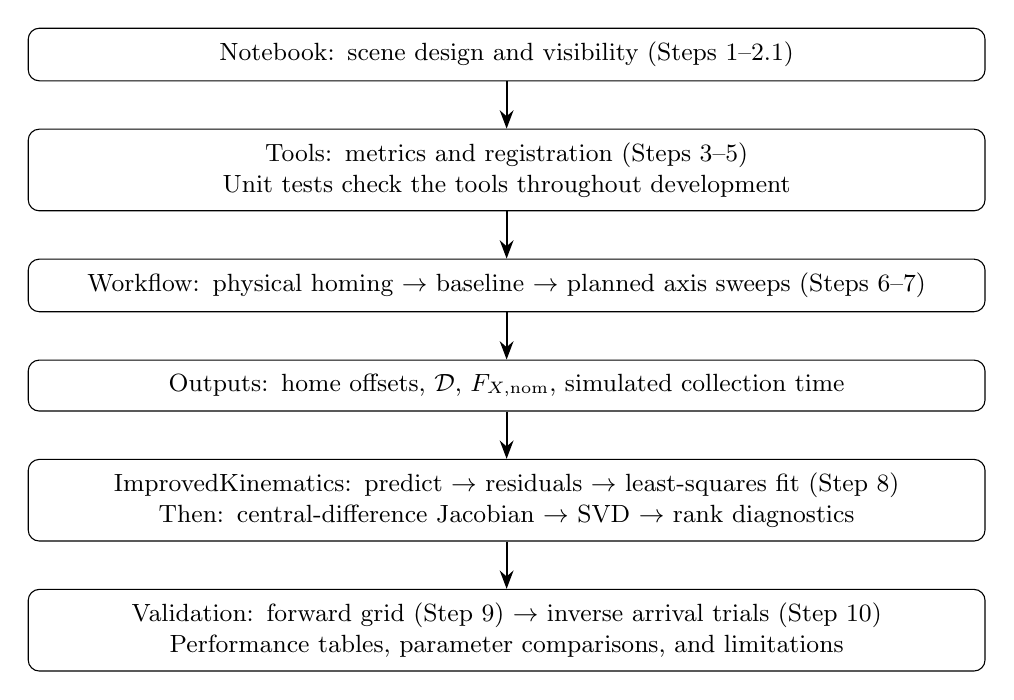
\begin{tikzpicture}[node distance=6mm,box/.style={draw,rounded corners,align=center,text width=11.8cm,font=\small,inner sep=5pt},arr/.style={-{Stealth},thick}]
\node[box] (a) {Notebook: scene design and visibility (Steps 1--2.1)};
\node[box,below=of a] (b) {Tools: metrics and registration (Steps 3--5)\\Unit tests check the tools throughout development};
\node[box,below=of b] (c) {Workflow: physical homing $\rightarrow$ baseline $\rightarrow$ planned axis sweeps (Steps 6--7)};
\node[box,below=of c] (d) {Outputs: home offsets, $\mathcal D$, $F_{X,\mathrm{nom}}$, simulated collection time};
\node[box,below=of d] (e) {ImprovedKinematics: predict $\rightarrow$ residuals $\rightarrow$ least-squares fit (Step 8)\\Then: central-difference Jacobian $\rightarrow$ SVD $\rightarrow$ rank diagnostics};
\node[box,below=of e] (f) {Validation: forward grid (Step 9) $\rightarrow$ inverse arrival trials (Step 10)\\Performance tables, parameter comparisons, and limitations};
\foreach \x/\y in {a/b,b/c,c/d,d/e,e/f}\draw[arr] (\x)--(\y);
\end{tikzpicture}
\caption{Program flow and dependency map. Calibration predicts in tracker coordinates; validation alone accesses hidden truth.}
\end{figure}

\begin{table}[H]\centering\footnotesize
\caption{Student modules and public functions.}
\begin{tabularx}{\linewidth}{@{}p{.19\linewidth}p{.36\linewidth}Y@{}}\toprule
Module & Functions & Inputs and outputs / responsibility\\\midrule
\texttt{metrics.py} & \texttt{frame\_error}; \texttt{summarize\_errors} & Two frames $\to$ angle/distance; error pairs $\to$ count, RMS and maxima.\\
\texttt{registration.py} & \texttt{register\_points}; \texttt{average\_frames}; \texttt{refine\_marker\_body} & Paired local/observed points $\to$ frame; frames $\to$ mean frame; tracked ordinary body $\to$ updated geometry.\\
\texttt{workflow.py} & \texttt{measure\_home\_offsets}; \texttt{plan\_calibration\_poses}; \texttt{collect\_calibration\_data}; \texttt{estimate\_base\_frame} & Robot $\to$ six offsets; robot/tracker/layout/accuracy $\to$ ordered joints; joints $\to$ \texttt{CalibrationData}; data/model $\to F_X$.\\
\texttt{kinematics.py} & \texttt{initial\_params}; \texttt{base\_frame}; \texttt{fwd\_kins}; \texttt{predict\_in\_tracker}; \texttt{inv\_kins} & Initialize corrections; parameters $\to$ base frame; joints $\to$ base/tracker pose; target/seed $\to$ joints.\\
\texttt{kinematics.py} & \texttt{residuals}; \texttt{fit}; \texttt{jacobian\_rank\_report}; \texttt{parameters\_report} & Data/parameters $\to$ weighted residuals; optimized parameters/diagnostics; singular values/rank/weak directions; physical parameter summaries.\\\bottomrule
\end{tabularx}\end{table}
The workflow helpers include the planner's local \texttt{append\_pose}, which validates and copies entries. The notebook helper \texttt{mbee\_markers\_world} applies nominal forward kinematics for visibility. Test helpers \texttt{random\_theta}, \texttt{random\_frame}, and the synthetic-fit test's \texttt{generate\_theta} create reproducible inputs. \texttt{CalibrationData} stores paired lists and collection duration. Supplied \texttt{robot.py}, simulation modules, frame types, and SE(3) helpers provide limits, motion timing, sampling, frame algebra, and exponential/log maps. The program outputs visibility counts, sample counts/times, fitting status/cost, rank, parameter comparisons, and forward/inverse performance tables.

\subsection{Supplied support files and test entry points}
The student-module table above covers our implemented calibration functions. The following inventory identifies the other assignment-local Python files; these support the algorithms rather than introducing additional fitted models.
\begin{table}[H]\centering\small
\caption{Supplied support modules, package initializers, and test files.}
\begin{tabularx}{\linewidth}{@{}p{.39\linewidth}Y@{}}\toprule
File (relative to \texttt{assignment2/}) & Responsibility\\\midrule
\texttt{src/robot.py} & Nominal forward/inverse kinematics, wrist branches, joint limits, state, and motion-time calculations.\\
\texttt{src/simulation/robot.py} & Creates the perturbed robot and simulates actual joint motion, physical homing, and validation-only truth access.\\
\texttt{src/simulation/tracker.py} & Creates the tracker/systematic field, manages tracked bodies, checks visibility, and provides clocked sampling.\\
\texttt{src/simulation/marker\_body.py} & Exposes body definition/placement, nominal-layout updates, recent-observation accessors, and a validation-only actual-frame helper.\\
\texttt{src/simulation/calibration\_body.py} & Enforces exact end-effector calibration-body construction and handles attachment/detachment.\\
\texttt{src/simulation/constants.py} & Stores supplied error bounds, noise levels, motion limits, timing, and acceptance targets.\\
\texttt{src/simulation/clock.py} & Implements the shared simulated elapsed-time accumulator.\\
\texttt{src/\_\_init\_\_.py} & Establishes imports and exposes the assignment's public robot, frame, and simulation API.\\
\texttt{src/simulation/\_\_init\_\_.py} & Re-exports simulation classes and functions.\\
\texttt{src/student/\_\_init\_\_.py} & Marks the student module package.\\
\texttt{tests/conftest.py} & Makes the assignment source importable during pytest execution.\\
\texttt{tests/test\_simulation.py} & Contains 23 supplied simulation/API checks.\\
\texttt{tests/test\_student.py} & Contains 14 checks of the student calibration components.\\\bottomrule
\end{tabularx}\end{table}
The notebook is the execution driver. Shared Assignment 1 tracker/marker code, the repository's \texttt{data\_types} package, and \texttt{uncertainty\_networks.se3} are dependencies rather than additional student implementations. Optional exploratory experiment scripts are separate from the main program and are described only in Appendix~\ref{app:fixed-parameters}.


\section{Validation Approach}
\subsection{Unit tests and current status}\label{sec:tests}
On October 25, 2026, running \texttt{python -B -m pytest -p no:cacheprovider tests -q} in the assignment directory produced \textbf{37 passed} in 1.23~s. All 23 supplied simulation tests and all 14 student tests passed.
\paragraph{Supplied simulator tests (23).}
The following list follows the order in \texttt{test\_simulation.py}; all tests passed.
\begin{enumerate}
\setlength{\itemsep}{0pt}
\item \textbf{Home FK:} checks identity orientation and position $(600,0,0)$ at zero nominal joints.
\item \textbf{Rotation convention:} checks axis-rotation signs against the SO(3) exponential map for $x,y,z$.
\item \textbf{Random nominal FK/IK:} recovers 100 seeded joint configurations through forward and inverse kinematics.
\item \textbf{Wrist branches:} checks that both nominal wrist solutions reproduce the requested rotation.
\item \textbf{Wrist singularity:} sets $\theta_5=\pi/2$ and checks that nominal IK followed by FK recovers the target rotation and position with \texttt{atol=1e-6}.
\item \textbf{Unreachable target:} checks that an out-of-workspace target raises an error and is reported unreachable.
\item \textbf{Joint limits:} checks rejection of commands beyond representative linear and rotary limits.
\item \textbf{Motion profiles:} checks long/short move times, zero-distance settling, and wrist motion time.
\item \textbf{Simulation clock:} checks that moves and samples advance time correctly, including sampling an empty scene.
\item \textbf{Homing and oracle:} checks physical zero, nonzero encoder offsets, and that reading a truth pose does not advance time.
\item \textbf{Initial state:} checks that a new robot starts at physical home while its encoders can read nonzero values.
\item \textbf{Joint-error bounds:} checks distortion magnitude/slope on 2000 configurations, the fixed first axis, and tilt bounds.
\item \textbf{Non-nominal truth:} checks that the simulated actual pose differs from nominal kinematics in a selected case.
\item \textbf{Frustum:} checks acceptance of visible points and rejection beyond the near, far, and side boundaries.
\item \textbf{Systematic field:} checks magnitude/gradient bounds at 300 random points and repeatability of each camera's field.
\item \textbf{Sample storage:} checks that a visible body returns four readings and a stored pose reasonably close to truth.
\item \textbf{No-jiggle frame:} checks five observations of an exact-layout body against its tracker-relative true pose.
\item \textbf{Invisible body:} checks that an out-of-view body returns no observation and clears its stored markers.
\item \textbf{Layout update:} checks that updating nominal geometry returns previous values, preserves truth, and rejects a changed point count.
\item \textbf{Tracking list:} checks adding/removing bodies and the returned previous tracking lists.
\item \textbf{Calibration-body rules:} checks the radius constraint, one-body restriction, and exact manufactured geometry.
\item \textbf{Attachment:} checks that the calibration body follows robot motion and disappears/reappears when detached/attached.
\item \textbf{Exact-body frame:} checks that the truth registration frame equals the actual placement for the exact calibration body.
\end{enumerate}

\paragraph{Student component tests (14).}
The following list follows the order in \texttt{test\_student.py}; all tests passed.
\begin{enumerate}
\setlength{\itemsep}{0pt}
\item \textbf{Known frame errors:} recovers a 0.1-rad angle and a 5-mm displacement from known examples.
\item \textbf{Frame invariance:} checks that a common left transform leaves the reported relative errors unchanged.
\item \textbf{Error statistics:} checks sample count, RMS, and maximum using distances 3 and 4.
\item \textbf{Known point registration:} recovers a seeded rigid transform from six exact corresponding point pairs.
\item \textbf{Insufficient points:} checks that registering only two pairs raises \texttt{ValueError}.
\item \textbf{Identical-frame average:} checks that averaging five identical frames returns the same frame.
\item \textbf{Proper mean rotation:} checks orthogonality and determinant $+1$ after averaging ten noisy-orientation frames.
\item \textbf{Marker refinement:} checks reduced rigidly aligned layout error after 30 readings and a 0.9-s simulated sampling cost.
\item \textbf{Base registration:} recovers a known $F_X$ from ten ideal synthetic joint/pose pairs.
\item \textbf{Pose plan:} checks that the plan is nonempty and every entry obeys joint limits and nominal marker visibility.
\item \textbf{Home offsets:} checks a six-component offset estimate from 20 homings against a further home encoder reading.
\item \textbf{Initial improved model:} checks nominal equivalence at ten joint configurations with zero offsets/corrections and checks initial base translation.
\item \textbf{Improved FK/IK:} checks ten pose round trips after small parameter perturbations, with errors below $10^{-6}$~mm and $10^{-8}$~rad.
\item \textbf{Synthetic fit:} fits 30 noise-free poses with one nonzero axis-tilt coefficient and checks ten held-out predictions using position/angle absolute tolerances $10^{-3}$~mm/$10^{-6}$~rad.
\end{enumerate}

The wrist-singularity test concerns the \emph{nominal} robot only; it does not establish robustness of calibrated IK near its own singular configurations. The Step 9 grid uses $\theta_5\in\{-1.3,0,1.3\}$ and excludes the nominal singular angles $\pm\pi/2$. Calibration-Jacobian rank analysis is a separate identifiability diagnostic, not a wrist-singularity test.

The refinement implementation now handles \texttt{most\_recent\_observed\_markers} correctly: its elements are already \texttt{vct3}, so it uses \texttt{list(observed)} without accessing a nonexistent \texttt{.p} member. The test passes both the aligned layout-error reduction check and the $30(0.03)=0.9$-s sampling-time check. The exact end-effector calibration body still does not require refinement, so this optional functionality is validated separately from the main calibration path.

Coverage limitations remain: the degenerate registration test checks two points, not every collinear/reflection case; the synthetic fit perturbs only one tilt coefficient; and the home-offset test uses one common tolerance across mixed joint units. Passing tests support the stated checks, not exhaustive correctness.

\subsection{Forward grid, inverse trials, and reproducibility}
The fixed forward levels are $(100,300,500)$ for joints 1 and 3, $(-200,0,200)$ for joint 2, $(-1.3,0,1.3)$ for joints 4 and 5, and $(-2,0,2)$ for joint 6. Their Cartesian product has 729 poses. These configurations combine joint motions, unlike the individual-axis calibration sweeps. All are visible under nominal geometry. They sample the interior and do not establish accuracy at all limits or every continuous pose.

Inverse trials use 40 grid configurations selected without replacement with \texttt{default\_rng(0)}. They use the corresponding joint configuration as an inverse-branch seed. This is a reachable-target arrival test, not a demonstration of global inverse convergence from arbitrary seeds. Nominal and improved moves are executed alternately, and reported testing time is their combined time.

For the report experiments, robot/systematic-field seeds are 1 and 2. Before each complete run, we set \texttt{np.random.seed(20261025)} to control the legacy random generator used by tracker sensor noise. The inverse target selector is separately fixed at seed 0. No observation noise is suppressed, no test thresholds are relaxed, and model parameters are not tuned using oracle values. The report reruns reset the simulation and recreate the scene; unit tests are run separately. The latest saved notebook fixes robot seed 1 but does not set this global sensor-noise seed. Its results are therefore a separate experiment, reported below rather than substituted into the controlled-seed tables. The notebook invokes pytest in a separate process, which does not consume the notebook process's random-number state.

\section{Results}
\subsection{Forward and inverse accuracy}
Tables below are populated from fresh complete report-validation executions, not a mixture of old notebook outputs. Position columns use mm and angle columns use rad.
\begin{table}[H]\centering\small
\caption{Accuracy for robot seed 1, sensor-noise seed 20261025.}
\begin{tabular}{@{}lrrrrrl@{}}\toprule
Model & $N$ & RMS pos. & Max pos. & RMS angle & Max angle & Pass\\\midrule

Forward nominal & 729 & 7.9997 & 16.6595 & 0.032604 & 0.054211 & No\\

Forward improved & 729 & 0.1125 & 0.1806 & 0.000276 & 0.000542 & Yes\\

Inverse nominal & 40 & 8.3271 & 14.1974 & 0.034464 & 0.054081 & No\\

Inverse improved & 40 & 0.1160 & 0.1584 & 0.000335 & 0.000662 & Yes\\

\bottomrule\end{tabular}\end{table}

\begin{table}[H]\centering\small
\caption{Accuracy for robot seed 2, sensor-noise seed 20261025.}
\begin{tabular}{@{}lrrrrrl@{}}\toprule
Model & $N$ & RMS pos. & Max pos. & RMS angle & Max angle & Pass\\\midrule

Forward nominal & 729 & 6.2394 & 13.7797 & 0.035322 & 0.054886 & No\\

Forward improved & 729 & 0.0651 & 0.1117 & 0.000263 & 0.000508 & Yes\\

Inverse nominal & 40 & 6.5867 & 12.9526 & 0.035585 & 0.053105 & No\\

Inverse improved & 40 & 0.0648 & 0.1119 & 0.000295 & 0.000537 & Yes\\

\bottomrule\end{tabular}\end{table}

\subsection{Simulated time, wall time, and optimizer diagnostics}
\begin{table}[H]\centering\small\caption{Timing and fit diagnostics for complete report runs.}\begin{tabular}{@{}lrr@{}}\toprule Quantity & Seed 1 & Seed 2\\\midrule

Baseline collection (simulated s) & 83.800 & 83.799\\

Main collection (simulated s) & 422.239 & 422.239\\

Total calibration (simulated s) & 506.411 & 506.412\\

Combined inverse testing (simulated s) & 1058.076 & 1057.680\\

Core pipeline wall time (s) & 12.755 & 10.373\\

Main samples / distinct configurations & 186 / 53 & 186 / 53\\

Move commands / tracker samples & 196 / 196 & 196 / 196\\

Fit cost & 201.7081 & 202.1531\\

Reported function evaluations & 24 & 19\\

Effective Jacobian rank & 33 / 34 & 33 / 34\\

Largest singular value & 4.469e+04 & 4.483e+04\\

Smallest singular value & 5.093e-06 & 4.633e-06\\

\bottomrule\end{tabular}\end{table}
Each run uses five physical homings, ten baseline moves, and 186 main-plan moves. The 196 tracker samples account for $196(0.03)=5.88$~s of simulated time; most calibration time is motion and settling. Total calibration minus baseline and main collection is approximately 0.4~s in these runs. No marker refinement or optional unit-test time is included. Forward evaluation reads the oracle without advancing the simulated clock.

The wall timer covers scene construction, baseline/main collection, fitting, rank and parameter reporting, and forward/inverse evaluation; it excludes unit tests and notebook startup. Both observed wall times are well below the handout's 600-s execution limit on this machine. They are not a grading-machine guarantee. The 900-s value printed by the notebook is a soft simulated-calibration budget in the supplied constants, not the handout's 10-minute real-execution limit. Combined inverse testing exceeds 900 simulated seconds because it includes both methods' actual motions; this is not a real-runtime violation.


\subsection{Latest saved notebook run}
The latest sequential notebook execution (cells numbered 1--13) reports 37 passing tests, successful fitting with cost 196.6188 and 17 reported function evaluations, and effective rank $33/34$. Robot seed is 1; the global tracker-noise seed is unspecified. This run is distinct from the controlled report-validation runs above.
\begin{table}[H]\centering\small
\caption{Latest saved notebook results; robot seed 1, sensor-noise seed unspecified.}
\begin{tabular}{@{}lrrrrrl@{}}\toprule
Model & $N$ & RMS pos. & Max pos. & RMS angle & Max angle & Pass\\\midrule
Forward nominal & 729 & 8.0570 & 16.7740 & 0.032624 & 0.054342 & No\\
Forward improved & 729 & 0.1096 & 0.1747 & 0.000198 & 0.000303 & Yes\\
Inverse nominal & 40 & 8.3863 & 14.2852 & 0.034463 & 0.054220 & No\\
Inverse improved & 40 & 0.1105 & 0.1541 & 0.000310 & 0.000715 & Yes\\
\bottomrule\end{tabular}\end{table}
The run collected 186 main samples at 53 distinct configurations in 422.2 simulated seconds. Total calibration took 506.4 simulated seconds; combined nominal/improved inverse testing took 1057.8873 simulated seconds. Both improved maximum errors satisfy the targets. No independent wall-time measurement was saved for this notebook run; the wall times in the earlier timing table belong only to the controlled report-validation runs.

\subsection{Parameter recovery and interpretation}
We report joint offsets, normalized polynomial coefficients and corresponding first-order scale factors, axes, pairwise axis angles, and tool correction. The first-order scale increment is $c_{k1}/s_k$, with total local scale at zero $1+c_{k1}/s_k$; away from zero the quadratic derivative also contributes. The fitted polynomial is not an exact decomposition of the simulator's systematic terms. In particular, physical-home encoder readings estimate an implicit near-home correction and should not be equated blindly with a named simulator constant.

Raw component subtraction of fitted axes/tilts/tool twists is gauge dependent. For debug comparisons we use
\begin{equation}
 \gamma_{ij}=\arccos\!\left(\operatorname{clip}(d_i^Td_j,-1,1)\right),\qquad
 e_\gamma=\max_{i,j}|\widehat\gamma_{ij}-\gamma_{ij}^{*}|.
\end{equation}
The maximum pairwise-axis angle differences were 0.01389 and 0.01467 degrees for seeds 1 and 2, respectively. The fit is not bounded to enforce the physical tilt/tool tolerances, so a gauge-equivalent solution can have large raw twists. This is a known limitation of the present parameterization, not evidence that the physical device actually has such large errors.

\subsection{Optional exploration of single-parameter constraints}
To investigate whether rank $33/34$ singles out one redundant parameter, we examined all 34 constraints on the same calibration data. At the original fitted point, 20 choices produced effective rank $33/33$ after removing the fixed parameter's Jacobian column. Fixing each parameter to zero and refitting gave 16 full-rank reduced Jacobians; 15 constraints preserved the baseline cost within 0.001, and 26 retained the forward-test accuracy targets. Three fits did not satisfy the optimizer's convergence criteria even after extended iterations, so their final costs are not treated as converged optima. Full results and qualifications are in Appendix~\ref{app:fixed-parameters}. This optional analysis did not alter the final implementation or its reported main calibration results.

\subsection{Error sources and limits of the result}
Both tested seeds meet the pointwise thresholds on the stated grid and inverse trials. This does not prove success for every seed or pose. Remaining errors include tracker systematic distortion, finite marker noise, uncertain home offsets, joint repeatability, and approximation error from quadratic joint maps. More repeated readings reduce independent noise but cannot remove a stationary systematic field. Dense sampling alone does not remove an exact coordinate gauge. Better future changes are a fixed gauge, a justified parameter scale/constraint policy, repeated-noise trials, boundary/random holdout tests, and a sampling design derived from the full error budget. Increasing polynomial degree without observability checks may worsen conditioning.

\section{Use of AI Tools}

We used Claude (Anthropic), through Claude Code, to check the notebook against the handout, discuss report requirements, and explain LaTeX formatting. We also used OpenAI Codex for notation and mathematical explanations, code suggestions and debugging for metrics/registration/workflow, review of the kinematic fitting and evaluation implementation, execution of validation experiments, and report drafting and revision. Codex also assisted with the independent 34-constraint exploration in the appendix; those experiments did not modify the main calibration code. AI assistance therefore included implementation and report preparation, not only proofreading. The module descriptions, equations, tests, and experimental qualifications in this report document the resulting implementation and checks.

Table~\ref{tab:prompts} gives representative types of requests used during development; it is illustrative rather than a complete interaction log.

\begin{table}[H]
\centering
\small
\caption{Representative requests to the AI tools during development.}
\label{tab:prompts}
\begin{tabular}{@{}rp{0.85\textwidth}@{}}
\toprule
\# & Prompt \\
\midrule
1  & ``Check if my notebook fits the assignment requirements.'' \\
2  & ``Summarize what this section of the handout is asking for.'' \\
3  & ``Explain what the mathematical approach section needs.'' \\
4  & ``Explain where this variable comes from.'' \\
5  & ``Where can I find this variable in the notebook?'' \\
6 & ``Write the algorithmic approach with pseudocode in this format.'' \\
7 & ``This table goes off the page, How do I fix it?.'' \\
8 & ``Why isn't this code block or image showing up in LaTeX?'' \\
9 & ``Look through the changes we made to the notebooks.'' \\
   & \dots \\
\bottomrule
\end{tabular}
\end{table}

\section{Who Did What}

\begin{table}[H]
\centering
\caption{Division of work.}
\label{tab:whodidwhat}
\begin{tabular}{@{}lcc@{}}
\toprule
Task & Bader Al-Salhabi & Yinxiang Luo \\
\midrule
Scene setup and visibility (Steps 1--2.1) & Main & Helped \\
Unit tests (Step 3)                      & Main & Helped \\
Metrics and registration (Steps 4--5)    & Helped & Main \\
Calibration workflow (Steps 6--7)        & Helped & Main \\
Kinematic fitting (Step 8)               & Main & Helped \\
Evaluation and performance (Steps 9--10) & Main & Helped \\
Report writing and editing              & Helped & Main \\
\bottomrule
\end{tabular}
\end{table}

Yinxiang primarily completed Steps 4--7 and led report preparation.
Bader primarily completed the remaining assignment components.
The authors assisted each other; use of AI tools is disclosed separately
in the preceding section.

\clearpage
\appendix
\section{Exploratory Single-Parameter Constraint Experiment}
\label{app:fixed-parameters}
This supplementary experiment explores identifiability; it is not an additional requirement of the assignment and is not used to replace the submitted model. We retained the original program and ran the experiment in an independent source-code copy. Robot/systematic-field seed 1 and global tracker-noise seed 20261025 produced one fixed data set of 186 calibration observations. Every case used this same data and the same 729 forward-validation configurations. Ground truth was accessed only for validation. No inverse-arrival trials were performed for these 34 alternatives.

\paragraph{Two distinct questions.}
Let $\beta_0$ be the original fitted vector and $J_0$ its $1116\times34$ Jacobian.
\begin{enumerate}
\item \textbf{Local column deletion (D):} fix $\beta_k$ at its fitted value $(\beta_0)_k$ and delete column $k$ from $J_0$. This checks local rank without changing the fitted point or residuals.
\item \textbf{Zero constraint and refitting (R):} fix $\beta_k=0$, initialize the other parameters from $\beta_0$, and optimize the remaining 33 parameters. Recompute the original residual function's central-difference Jacobian at the resulting point, then remove its fixed column. A zero constraint can restrict the attainable model; it is not equivalent to merely choosing the original fitted value.
\end{enumerate}
The reduced fits use trust-region least squares with \texttt{x\_scale='jac'} and \texttt{ftol=xtol=gtol=1e-9}. The initial evaluation cap is 100; cases reaching it are continued for up to 1000 additional evaluations. The batched residual calculation used to accelerate these fits was checked against the original residual function at the baseline, ten perturbed parameter vectors, and every final solution (absolute tolerance $2\times10^{-8}$, relative tolerance $10^{-9}$); the initial maximum difference was $1.89\times10^{-12}$. Jacobian diagnostics use the original function. The original baseline uses the main program's optimizer settings, so very small cost reductions can reflect tighter stopping criteria rather than added information.

\paragraph{Rank definition and baseline.}
Ranks use $\sigma_i>10^{-6}\sigma_{\max}$, as in the main code. Both D and R matrices have 33 columns, so full column rank means 33. The baseline has rank $33/34$, cost $C_0=201.708060576$, maximum position error 0.180556622~mm, and maximum angle error 0.000541673~rad. For the original Jacobian, $\sigma_{\max}=44689.896$ and $\sigma_{\min}=5.093\times10^{-6}$. Changing the relative threshold to $10^{-5}$ or $10^{-7}$ changes the number of full-rank D cases from 20 to 18 or 21, respectively. With column-unit-norm scaling and the $10^{-6}$ relative threshold, 20 D cases are full rank. These are effective numerical ranks, not exact symbolic rank proofs.

\paragraph{Reading the table.}
Indices below are one-based; the code's array index is one less. Parameter names follow the 34-entry layout in the main report. $|v_k|$ is the magnitude of the corresponding component of the original smallest right singular vector, in the raw parameter coordinates. It depends on units and parameterization and is not a unit-independent ranking of ``redundancy.'' $\Delta C=C_{\mathrm{fixed}}-C_0$. Position and angle columns are maximum errors after zero-constrained refitting, in mm and rad. ``Conv.'' records optimizer convergence; ``Pass'' records both forward maximum-error targets, independently of convergence.

\begingroup
\setlength{\tabcolsep}{3pt}
\footnotesize
\begin{longtable}{@{}rlrccrrrcc@{}}
\caption{All 34 single-parameter constraints on identical calibration data. D and R ranks are out of 33.}\label{tab:all-fixed-parameters}\\
\toprule
\# & Fixed parameter & $|v_k|$ & D & R & $\Delta C$ & Max mm & Max rad & Conv. & Pass\\
\midrule
\endfirsthead
\multicolumn{10}{l}{\tablename\ \thetable\ (continued)}\\
\toprule
\# & Fixed parameter & $|v_k|$ & D & R & $\Delta C$ & Max mm & Max rad & Conv. & Pass\\
\midrule
\endhead
\midrule
\multicolumn{10}{r}{Continued on next page}\\
\endfoot
\bottomrule
\endlastfoot
1 & \texttt{base\_alpha\_x} & 3.22e-01 & 33 & 33 & 0.0000 & 0.18056 & 0.000542 & Yes & Yes\\
2 & \texttt{base\_alpha\_y} & 8.97e-04 & 33 & 33 & 0.0000 & 0.18056 & 0.000542 & Yes & Yes\\
3 & \texttt{base\_alpha\_z} & 2.17e-04 & 33 & 33 & 0.0000 & 0.18056 & 0.000542 & Yes & Yes\\
4 & \texttt{base\_rho\_x} & 2.43e-04 & 32 & 32 & 15.0345 & 0.20506 & 0.000656 & No & No\\
5 & \texttt{base\_rho\_y} & 1.75e-02 & 33 & 33 & 27.2795 & 0.50507 & 0.000586 & No & No\\
6 & \texttt{base\_rho\_z} & 6.13e-01 & 33 & 33 & 0.0000 & 0.18056 & 0.000542 & Yes & Yes\\
7 & \texttt{d2\_phi\_x} & 3.22e-01 & 33 & 33 & 0.0000 & 0.18056 & 0.000542 & Yes & Yes\\
8 & \texttt{d2\_phi\_z} & 3.77e-05 & 33 & 32 & 9.9852 & 0.42252 & 0.000546 & Yes & No\\
9 & \texttt{d3\_phi\_x} & 3.22e-01 & 33 & 33 & 0.0000 & 0.18056 & 0.000542 & Yes & Yes\\
10 & \texttt{d3\_phi\_y} & 1.09e-04 & 33 & 32 & 134.2302 & 1.24700 & 0.000560 & Yes & No\\
11 & \texttt{n4\_phi\_y} & 3.19e-03 & 33 & 33 & 0.0000 & 0.18056 & 0.000542 & Yes & Yes\\
12 & \texttt{n4\_phi\_z} & 2.52e-03 & 33 & 33 & 0.0000 & 0.18056 & 0.000542 & Yes & Yes\\
13 & \texttt{n5\_phi\_x} & 3.22e-01 & 33 & 33 & 0.0000 & 0.18056 & 0.000542 & Yes & Yes\\
14 & \texttt{n5\_phi\_z} & 6.95e-04 & 33 & 32 & 5311.2756 & 6.40521 & 0.012413 & Yes & No\\
15 & \texttt{n6\_phi\_x} & 3.22e-01 & 33 & 33 & 0.0000 & 0.18056 & 0.000542 & Yes & Yes\\
16 & \texttt{n6\_phi\_y} & 2.63e-04 & 33 & 32 & 897.6863 & 2.62060 & 0.004239 & Yes & No\\
17 & \texttt{tool\_alpha\_x} & 3.22e-01 & 33 & 33 & 0.0000 & 0.18056 & 0.000542 & Yes & Yes\\
18 & \texttt{tool\_alpha\_y} & 1.15e-04 & 33 & 33 & 0.0000 & 0.18056 & 0.000542 & Yes & Yes\\
19 & \texttt{tool\_alpha\_z} & 7.93e-04 & 33 & 33 & 0.0000 & 0.18056 & 0.000542 & Yes & Yes\\
20 & \texttt{tool\_rho\_x} & 7.30e-05 & 32 & 32 & 4.5000 & 0.27537 & 0.000511 & No & No\\
21 & \texttt{tool\_rho\_y} & 3.51e-02 & 33 & 33 & 0.0000 & 0.18056 & 0.000542 & Yes & Yes\\
22 & \texttt{tool\_rho\_z} & 3.94e-02 & 33 & 33 & 0.0000 & 0.18056 & 0.000542 & Yes & Yes\\
23 & \texttt{joint1\_c1} & 5.19e-08 & 32 & 32 & 0.1231 & 0.18589 & 0.000543 & Yes & Yes\\
24 & \texttt{joint1\_c2} & 1.92e-07 & 32 & 32 & 0.0011 & 0.18048 & 0.000542 & Yes & Yes\\
25 & \texttt{joint2\_c1} & 2.31e-09 & 32 & 32 & 0.3148 & 0.20684 & 0.000542 & Yes & No\\
26 & \texttt{joint2\_c2} & 7.77e-09 & 32 & 32 & 0.0029 & 0.17786 & 0.000542 & Yes & Yes\\
27 & \texttt{joint3\_c1} & 4.30e-09 & 32 & 32 & 0.3377 & 0.18063 & 0.000540 & Yes & Yes\\
28 & \texttt{joint3\_c2} & 3.54e-08 & 32 & 32 & 0.0381 & 0.18044 & 0.000541 & Yes & Yes\\
29 & \texttt{joint4\_c1} & 3.62e-12 & 32 & 32 & 0.3970 & 0.17482 & 0.000527 & Yes & Yes\\
30 & \texttt{joint4\_c2} & 7.20e-13 & 32 & 32 & 0.2630 & 0.17593 & 0.000504 & Yes & Yes\\
31 & \texttt{joint5\_c1} & 3.88e-11 & 32 & 32 & 0.1110 & 0.17949 & 0.000555 & Yes & Yes\\
32 & \texttt{joint5\_c2} & 1.23e-12 & 32 & 32 & 0.1272 & 0.17917 & 0.000532 & Yes & Yes\\
33 & \texttt{joint6\_c1} & 2.91e-11 & 32 & 32 & 1.6842 & 0.16328 & 0.000416 & Yes & Yes\\
34 & \texttt{joint6\_c2} & 2.00e-11 & 32 & 32 & 0.3052 & 0.18024 & 0.000474 & Yes & Yes\\
\end{longtable}
\endgroup

\paragraph{Interpretation and limits.}
For example, fixing \texttt{base\_alpha\_x}, \texttt{d2\_phi\_x}, or \texttt{tool\_alpha\_x} to zero separately gives rank $33/33$ and preserves cost and forward prediction to the displayed precision. Thus no single parameter is uniquely identified as ``the redundant parameter.'' These are alternative constraints intersecting the same weak direction. In contrast, fixing \texttt{n5\_phi\_z}=0 produces a maximum position error of approximately 6.405~mm even though deleting its column at the original fitted point gives rank 33. This illustrates the distinction between local identifiability and the effect of imposing a particular parameter value.

The three non-converged cases are \texttt{base\_rho\_x}, \texttt{base\_rho\_y}, and \texttt{tool\_rho\_x}; they reached 1100 cumulative reported function evaluations. Their rows describe final iterates, not proven constrained optima. The other 31 fits satisfied the stopping criteria, which still do not guarantee global optimality. Some rank-deficient alternatives retain acceptable forward accuracy because prediction and parameter uniqueness are different objectives. The experiment concerns one calibration data set and one parameterization; it does not establish robustness across arbitrary seeds, coordinate conventions, or inverse-kinematics singularities. For these reasons, the exploration is reported here without changing the main model.

\clearpage
\begin{thebibliography}{9}
\bibitem{handout} R. H. Taylor, ``Assignment 2 -- CIS I (601.455/655),'' Johns Hopkins University, October 15, 2026, pp. 1--7.
\bibitem{frames} R. H. Taylor, ``Basic Mathematical Methods for CIS: Cartesian Coordinates, Points, and Transformations,'' CIS I lecture material, local file \texttt{lectures/week2/frames.pdf}.
\bibitem{rigid} R. H. Taylor, ``Computing rigid 3D--3D transformations from point and line pairs,'' CIS I lecture material, local file \texttt{lectures/week3/rigid3d3dcalculations.pdf}.
\bibitem{shi_arun} J. Shi, ``Arun's Method for 3D Registration,'' online tutorial and Python implementation, \url{https://jingnanshi.com/blog/arun_method_for_3d_reg.html}, accessed October 25, 2026.
\bibitem{calibration} R. H. Taylor, ``Calibration,'' CIS I lecture material, local file \texttt{lectures/week4/calibration.pdf}.
\bibitem{cv} EN.601.661 Computer Vision, ``4C: Camera Calibration and Photogrammetry,'' Fall 2026 course slides, slide 40, nonlinear refinement.
\bibitem{notes} Y. Luo, annotated Assignment 2 and handwritten calibration analysis, October 2026, supplied 16-page annotated PDF, pp. 8--16. Derivations in this report correct notation and distinguish numerical rank from exact identifiability.
\end{thebibliography}

\end{document}
